% !TeX root = report.tex
\documentclass[12pt]{article}
\usepackage[utf8]{inputenc}
\usepackage{geometry}
\geometry{a4paper, margin=1in}
\usepackage{graphicx}
\usepackage{amsmath}
\usepackage{hyperref}
\usepackage{float}
\usepackage{listings}
\usepackage[table]{xcolor}

\title{The Open Brew: A Decentralized Cooperative Platform for Coffee Communities}
\author{Gökay Temizkan\\
Bogazici University, Department of Computer Engineering\\}
\date{\today}

\begin{document}

\maketitle

\begin{abstract}
The Open Brew is a decentralized, open, and cooperative social media platform designed to connect coffee enthusiasts, farmers, roasters, and baristas worldwide. This report outlines the model of the Open Brew platform, including its social, technical, and cooperative characteristics. The platform aims to make high-quality coffee more accessible and sustainable for all by promoting four main pillars: access, direct sourcing, home brewing, and education. The report also presents a methodology for analyzing the social dynamics of the Open Brew community using network analysis techniques and hypothesis testing. Finally, a use case is provided to demonstrate how the Open Brew platform can be used to analyze user interactions and engagement within the community.
\end{abstract}

\section{Introduction and Motivation}
\label{section:introduction_and_motivation}
Coffee is an integral part of modern life, with over 2.25 billion cups consumed worldwide every day \cite{Paterek2024CoffeeLI}. The coffee industry is a multi-billion-dollar industry that employs millions of people worldwide, from farmers to roasters to baristas \cite{Paterek2024CoffeeLI}. With its rich history, cultural significance, and economic impact, coffee has become an essential part of our daily lives \cite{Paterek2024CoffeeLI}.

Coffee has also played a significant role in the development of various societies and economies. In the United States, for instance, coffee became an integral part of American culture, particularly during the American Revolution \cite{Paterek2024CoffeeLI}. The Boston Tea Party, which led to the American Revolution, was actually a protest against the British government's taxation of tea, which made coffee an even more popular beverage in America \cite{Paterek2024CoffeeLI}. In fact, the United States is one of the world's largest consumers of coffee, with over 400 million cups consumed every day \cite{Paterek2024CoffeeLI}.

In terms of its economic impact, coffee has had a significant impact on various countries and communities. In Nicaragua, for example, smallholder cooperative leaders working in partnership with a California-based small-scale roasting company pioneered an alternative approach to confronting the post-1999 coffee crisis \cite{Bacon2013QualityRS}. They built coffee tasting laboratories and integrated grassroots organizing efforts to create a national smallholder cooperative association that dramatically improved the quality, consistency, and prices from of the coffee they exported \cite{Bacon2013QualityRS}.

Being such an integral part of modern life, there exist several movements and communities that focus on coffee, such as Third Wave Coffee, Fair Trade Coffee, Direct Trade Coffee etc. These movements aim to improve the quality of coffee, ensure fair compensation for farmers, and promote sustainable practices in the coffee industry. However, there exist a broader need for a community that connects all stakeholders in the coffee industry, including farmers, roasters, baristas, and enthusiasts that aims to make coffee more accessible, sustainable, and enjoyable for everyone.

To address this broader need for connection and collaboration across the coffee industry, we introduce the Open Brew community: a decentralized, open, and cooperative social media platform designed to unite coffee enthusiasts and professionals. Building on the foundations laid by existing movements, Open Brew seeks to make high-quality coffee more accessible and sustainable for all. The platform's mission is fourfold: to facilitate access to excellent coffee at reasonable prices outside the home, enable direct sourcing of specialty beans without intermediaries, empower individuals to brew exceptional coffee themselves, and promote education and awareness about all aspects of quality coffee. By integrating these pillars, Open Brew aims to foster a vibrant, inclusive culture where everyone can enjoy, understand, and actively participate in the world of coffee.

\section{The Model}
\label{section:the_model}
The Open Brew community is designed to be a decentralized, open, and cooperative social media platform that connects coffee enthusiasts, farmers, roasters, and baristas worldwide. The platform is built on the principles of decentralization, openness, and cooperation, allowing users to share their knowledge, experiences, and resources freely.

\subsection{The Social Characteristics of the Open Brew}
\label{subsection:social_characteristics_of_the_open_brew}
The open brew community includes all the stakeholders in the coffee industry (except large corporations such as Starbucks), listed as below:

\begin{itemize}
    \item Coffee Farmers: Individuals or cooperatives that grow and harvest coffee beans.
    \item Roasters: Professionals or businesses that roast green coffee beans to create the final product.
    \item Baristas: Skilled individuals who prepare and serve coffee beverages, often in cafes or restaurants.
    \item Enthusiasts: Coffee lovers who enjoy brewing and tasting coffee at home or in social settings.
    \item Educators: Individuals or organizations that provide training and resources on coffee brewing, tasting, and appreciation.
\end{itemize}

The large cooperations are planned to be excluded from the Open Brew community to ensure that the platform remains focused on small-scale, sustainable practices and to prevent the influence of corporate interests on the community's values and goals.

\subsection{The Technical Characteristics of the Open Brew}
\label{subsection:technical_characteristics_of_the_open_brew}
The technical characteristics of the Open Brew social network is modeled after Mastodon, a Decentralized Online Social Network (DOSN) that utilizes open-source software allowing users to create and host their own independent servers, known as instances. These instances are interconnected in a transparent manner through the use of specific communication protocols, forming a cooperative model called the Fediverse or federated universe \cite{la2022information}.

Technically, as in Mastodon, The Open Brew adopts the ActivityPub protocol, which enables both client-to-server and server-to-server communication, facilitating seamless interaction between users across different Fediverse instances without the need for multiple subscriptions, similar to email. This protocol also allows The Open Brew community to interact with other services within the Fediverse including Mastadon.

One of the most important technical features for achieving the community's goals is the ability to extract data about user relations. This can be accomplished using the publicly available REST APIs provided by the platform, which allow for programmatic access to user, post, and relationship data. By relying on authenticated requests, the platform ensures that privacy is respected and that only authorized data is accessed, avoiding the need for scraping tools that may violate user consent or platform policies. This approach enables researchers and community members to analyze social connections, engagement patterns, and the overall health of the network while maintaining transparency and user trust.

\subsection{The Social Media Model of the Open Brew}
\label{subsection:social_media_model_of_the_open_brew}
The Open Brew platform is inspired by Reddit platform in terms of its social media model. It allows users to create and share content, engage in discussions, and build communities around specific topics related to coffee. These dedicated spaces are called "brews" in Open Brew, analogous to Reddit's "subreddits". Each brew focuses on a specific topic or interest within the coffee domain.

To promote the four main pillars of the aimed Open Brew movement, four brews are created and promoted at the starting phase of the platform, each dedicated to one of the pillars:

\begin{itemize}
    \item Brew for Access: Focused on making high-quality coffee accessible at reasonable prices outside the home.
    \item Brew for Direct Sourcing: Dedicated to enabling direct sourcing of specialty beans without intermediaries.
    \item Brew for Home: Aimed at empowering individuals to brew exceptional coffee themselves.
    \item Brew for Education: Focused on promoting education and awareness about all aspects of quality coffee.
\end{itemize}

These brews serve as hubs for users to share their knowledge, experiences, and resources related to each pillar. In the later phases of the platform, additional brews are expected to be created to cover other aspects of the movement by the community members.

Again, inspired by Reddit, the Open Brew platform allows users to upvote or downvote content, which helps surface the most relevant and engaging posts within each brew. This voting system encourages quality contributions and encourages a sense of community ownership over the content shared on the platform.

In the platform, text content is the primary form of communication. The main reason for this is to encourage users to share their thoughts, ideas, and experiences. An additional favour of this decision is to allow network analysis to be conducted more easily, as text data is generally easier to process and analyze than multimedia content. However, the platform also supports multimedia content such as images and videos.

An example of a post in the Open Brew platform will look like the following:
\begin{figure}[H]
    \centering
    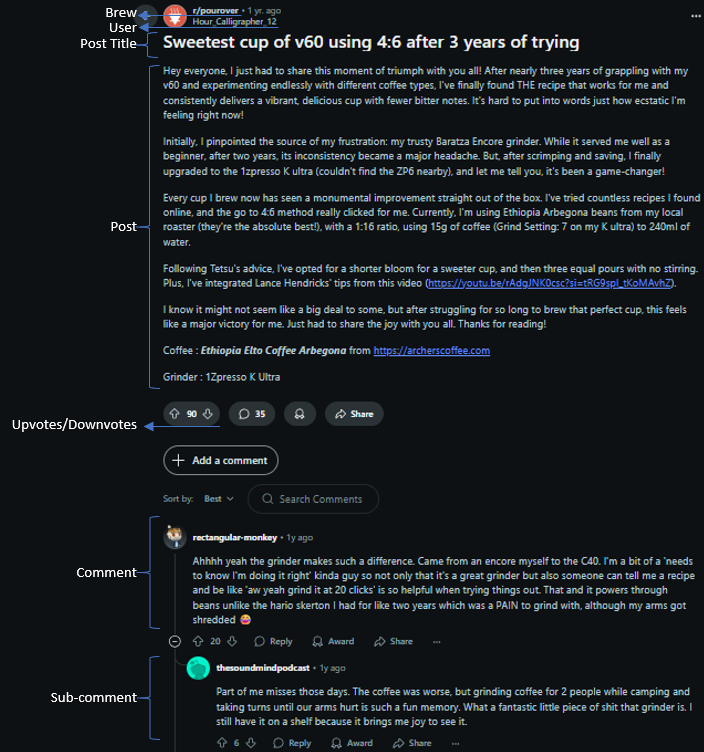
\includegraphics[width=0.9\textwidth]{example_post.png}
    \caption{An example post in the Open Brew platform (derived from Reddit).}
    \label{fig:example_post}
\end{figure}

Figure \ref{fig:example_post} shows an example post in the Open Brew platform derived from Reddit \cite{reddit2024sweetestv60}. The post includes a title, content, and options for users to upvote or downvote the post. Users can also comment on the post, allowing for discussions and interactions within the community.

\subsection{Cooperative Characteristics of the Open Brew}
\label{subsection:cooperative_characteristics_of_the_open_brew}
The Open Brew platform is designed to be a cooperative social media platform. It allows and inspires users to collaborate and work together towards common goals.

One important aspect of the cooperative nature of the Open Brew platform is the different roles of users. The users are able to identify themselves as farmers, roasters, baristas, enthusiasts, or educators as defined in Section \ref{subsection:social_characteristics_of_the_open_brew}. These roles will be visible to other users, allowing them to understand the expertise and interests of each user.

This role-based system encourages users to collaborate and share their knowledge and resources with others in the community. For example, farmers can share their experiences and insights on growing coffee beans, while roasters can provide tips on roasting techniques. Baristas can share their expertise on brewing methods, and enthusiasts can share their passion for coffee. Educators can provide training and resources to help others improve their coffee knowledge and skills.

\section{Method}
\label{section:method}
The Open Brew platform is designed to be a collaborative platform that has four main pillars, each of which is designed to address a specific aspect of the coffee community: access, direct sourcing, home brewing, and education. In this section, we outline the methodology used to analyze and model the Open Brew platform, ensuring that it meets the needs of its diverse user base while promoting collaboration and knowledge sharing.

\subsection{Approach}
\label{subsection:approach}
The approach of this project is to start a movement with the four main goals of the Open Brew platform, as described in Section \ref{section:introduction_and_motivation} by creating a federated social media platform and a community around it. The platform design and feature specifications are discussed in detail in Section \ref{section:the_model}. Next, we will focus on the data collection and analysis of the Open Brew platform. Finally, we will test the hypotheses proposed in Section \ref{subsection:hypotheses} to understand the social dynamics of the Open Brew community and how users engage with each other and the content shared on the platform.

\subsection{Data Collection}
\label{subsection:data_collection}
The data collection process for the Open Brew platform involves gathering information from various sources, including user-generated content, interactions, and relationships within the community. The data will be collected using the publicly available APIs provided by the platform. These APIs will be developed modelling Mastodon REST APIs \cite{mastodonAPI}.

The data collection will be handled in a similar approach to the one used in the study "Information consumption and boundary spanning in decentralized online social networks: the case of mastodon users" \cite{la2022information}. The data collection will be conducted using a privacy-friendly crawler that utilizes authenticated requests to ensure compliance with privacy requirements. The crawler will focus on collecting data from instances that allow accountable requests via The Open Brew APIs, avoiding the use of scraping tools.

The data extraction will begin with identifying key "brews" including but not limited to the four initial brews created: Brew for Access, Brew for Direct Sourcing, Brew for Home, and Brew for Education. Information will be gathered from the timelines of these brews to discover community characteristics and user interactions. A breadth-first search method will be employed to find new connections and consequently more users.

The data collection process will result in a dataset that contains information about anaonymized user interactions, relationships, and the overall structure of the Open Brew community. This dataset will be used to analyze the social dynamics of the platform, identify key players, and understand how users engage with each other and the content shared on the platform.

An example of the data collected from the Open Brew platform is provided in Appendix \ref{lst:openbrew_data}.

As provided in the example, the data includes information about users, posts, and comments. Each user has an ID, username, and role (e.g., enthusiast, roaster). Posts contain content, timestamps, upvotes, downvotes, and comments. Comments also include user IDs, content, timestamps, upvotes, downvotes, and nested comments.

In addition to detailed data extraction, the platform will provide a dedicated API endpoint to extract basic aggregate statistics for a requested time period. This API will return the number of users, number of brews, number of posts, and number of comments within the specified interval. This feature enables efficient monitoring of community growth and activity over time without requiring full data dumps. An example query output from this API is provided in Appendix \ref{lst:openbrew_basic_stats}.

\subsection{Data Analysis}
\label{subsection:data_analysis}
The data analysis will be conducted using network analysis techniques to understand the structure and dynamics of the Open Brew community.

\subsubsection{Social Network Analysis (SNA)}
\label{subsubsection:social_network_analysis}
Social Network Analysis (SNA) will be employed to analyze the relationships and interactions between users within the Open Brew platform. SNA allows us to visualize and quantify the connections between users, identify key players, and understand how information flows within the community.

Its planned to create two separate dynamic network graphs that will represent votes (upvotes and downvotes) and comments between users in the Open Brew community. Both of the graphs will be directed graphs where nodes represent users and edges represent votes or comments made by one user on another user's post or comment. The characteristics of the network graphs will be as follows:

\begin{itemize}
\item Votes Graph:
    \begin{itemize}
    \item Nodes: Represent users in the Open Brew community.
    \item Node Attributes: Include user roles (e.g., farmer, roaster, barista, enthusiast, educator).
    \item Edges: Represent votes (upvotes and downvotes) between users.
    \item Edge Weights: Represent the number of upvotes minus downvotes made by one user on another user's post.
    \item Edge Direction: Indicates the direction of the vote (from voter to post author).
    \item Edge Attributes: Include timestamps allowing for temporal analysis of interactions. It should be noted that, as data collection does not include votes' timestamps, the edge will represent the time of the post or comment that the vote is related to.
    \end{itemize}

\item Comments Graph:
    \begin{itemize}
    \item Nodes: Represent users in the Open Brew community.
    \item Node Attributes: Include user roles (e.g., farmer, roaster, barista, enthusiast, educator).
    \item Edges: Represent comments made by one user on another user's post or comment.
    \item Edge Weights: Represent the number of comments made by one user on another user's post or comment.
    \item Edge Direction: Indicates the direction of the comment (from commenter to post or comment author).
    \item Edge Attributes: Include timestamps allowing for temporal analysis of interactions.
    \end{itemize}

\item Common Features:
    \begin{itemize}
    \item Graph Layout: The graph will be laid out in a way that visually represents the relationships between users, with clusters of users who frequently interact with each other.
    \item Graph Dynamics: The graph will be dynamic, allowing for the visualization of changes in user interactions over time.
    \item Visualization: The graph will be visualized using network visualization tools, such as Gephi or NetworkX, to provide insights into the community's dynamics and relationships.
    \end{itemize}
\end{itemize}

\subsubsection{Temporal Network Analysis}
\label{subsubsection:temporal_network_analysis}
Temporal analysis is vital in Social Network Analysis because human social networks are fundamentally dynamic. Many critical social processes, such as the spread of influence or diffusion of information, occur over time and require temporal considerations \cite{robins2013tutorial}.

As mentioned in the Section \ref{subsubsection:social_network_analysis}, the data collection will include timestamps for posts, and comments. This temporal information will be crucial for understanding how the Open Brew community evolves over time.

The analysis is planned to employed on three periods: the first month after the launch of the platform, the first three months, and the first year. This will allow us to observe how user interactions change over time, identify trends in community growth, and understand how different user roles engage with each other.

Temporal analysis in the context of the Open Brew community can focus on several key aspects:

\begin{itemize}
    \item Growth of the Community: Track the increase in the number of users, posts, comments, and brews over time to understand adoption and engagement trends.
    \item Evolution of User Interactions: Analyze how the frequency and patterns of interactions change across different time periods.
    \item Emergence of Influential Users and Brews: Identify when and how certain users or brews become central or influential within the network.
    \item Retention and Churn: Measure user retention rates and identify patterns in user departure or inactivity over time.
\end{itemize}

\subsubsection{Role-Based Interaction Patterns}
\label{subsubsection:role_based_interaction_patterns}
Role-based analysis is important for understanding how different positions or functions held by participants within a network influence interaction patterns over time. This analysis could assess tendencies towards "homophily" (interacting with those of the same role) or "heterophily" (interacting with those of a different role). The importance lies in determining if roles create structural preferences or barriers to communication \cite{stepanyan2014culture}.

Here, we will analyze how different user roles (farmers, roasters, baristas, enthusiasts, educators) interact within the network. Metrics such as assortativity, role-based centrality, and cross-role engagement will be examined to understand collaboration and knowledge sharing across roles.

\subsubsection{Key Users and Influencers}
\label{subsubsection:key_users_and_influencers}
Determining key users within a network is essential, because it relates to the phenomenon of "preferential attachment". This effect, often described as "the rich get richer," signifies that participants who are already highly active and have many connections tend to attract even more connections over time. Identifying these users, who become disproportionately well-connected, reveals patterns like the "power-law distribution of degree centrality" within the network. Understanding who these key users are and the dynamics by which they become central is crucial because a strong preferential attachment pattern can lead to a "growing disparity between participants", potentially making it less likely for less active individuals to engage \cite{stepanyan2014culture}.

Therefore, determining key users allows educators and designers to recognize potential structural inequalities in communication and consider timely interventions, such as adjusting facilitation methods, to help "balance the interaction" and encourage broader participation.

In this study, it is crucial to sustainably identify key users and influencers within the Open Brew community. This will be achieved through a combination of SNA metrics, such as degree centrality, betweenness centrality, and eigenvector centrality. These metrics will help identify users who are not only well-connected but also play significant roles in facilitating communication and information flow within the network.

\subsection{Hypotheses}
\label{subsection:hypotheses}
The following hypotheses are proposed to guide the analysis of the Open Brew community:
\begin{itemize}
    \item H1: The Open Brew network will show preferential attachment, with a few users becoming key influencers.
    \item H2: Users will interact more across different roles (heterophily) than within the same role.
    \item H3: Community activity (brews, posts, comments) will increase over time, possibly exponentially.
\end{itemize}

\section{Use Case}
\label{section:use_case}
In this section, we will present a use case for the Open Brew platform, demonstrating how it can be used to make way towards the four main pillars of the Open Brew movement (Section \ref{section:introduction_and_motivation}) and how it can be used to analyze the social dynamics of the community.

For this example, we assume that the Open brew platform has been launched and run for a period of one year, and the data collection has been completed as described in Section \ref{subsection:data_collection}.

On the collected data, we test the hypotheses proposed in Section \ref{subsection:hypotheses} to understand the social dynamics of the Open Brew community and how users engage with each other and the content shared on the platform.

\subsection{Creating the Network Graphs}
\label{subsection:creating_network_graphs}
The first step in the analysis is to create the network graphs representing votes and comments between users in the Open Brew community, as described in Section \ref{subsubsection:social_network_analysis}. The graphs will be created using the collected data, and the nodes will represent users while the edges will represent votes or comments made by one user on another user's post or comment.

The network graphs will be created using Python and the NetworkX library, which provides tools for creating, manipulating, and analyzing complex networks. The graphs will be visualized using Gephi to provide insights into the community's dynamics and relationships.

The pseudocode for constructing the network graphs is provided in Appendix \ref{sec:pseudocode_for_constructing_network_graphs}. The full code can be found in the GitHub repository of the project.

\subsection{Testing the Hypotheses}
\label{subsection:testing_hypotheses}
All three hypotheses proposed in Section \ref{subsection:hypotheses} are significant for understanding the social dynamics of the Open Brew community and assure that the platform is designed to meet the needs of its diverse user base while promoting collaboration and knowledge sharing.

In this section, we will report how we test the hypotheses using the network graphs created in Section \ref{subsection:creating_network_graphs}. The tests will be conducted using statistical methods and network analysis techniques to validate or refuse the hypotheses.

\subsubsection{Testing H1: Power-Law Distribution}
\label{subsubsection:testing_h1_power_law_distribution}
According to Stepanyan et al. \cite{stepanyan2014culture}, the existence of preferential attachment within a social network can be demonstrated using correlational analysis for degree centrality.

Accordingly, to test for preferential attachment (H1), we will calculate the Pearson correlation between users' degree centrality at three months and at the end of the observation period. A high correlation indicates that well-connected users tends to remain central, supporting preferential attachment.

\subsubsection{Testing H2: Role-Based Interaction Patterns}
\label{subsubsection:testing_h2_role_based_interaction_patterns}
Homophily is defined as "the principle that a contact between similar people occurs at a higher rate than among dissimilar people". This means that individuals tend to interact more frequently with others who share similar characteristics. Heterophily on the other hand indicates a tendency towards interaction across different types of actors \cite{stepanyan2014culture}.

To investigate role-based interaction patterns, we will utilize "assortativity coefficient". Assortativity coefficient is a measure used in Social Network Analysis (SNA) to quantify the tendency of nodes (or vertices) in a network to connect with other nodes of similar characteristics, such as degree, strength, or other node-specific attributes \cite{Wang2016TheHR}. It measures the correlation between the degrees or strengths of nodes at the ends of an edge, and it is often used to understand the structure and evolution of networks \cite{Wang2016TheHR}.

We will calculate the assortativity coefficient for the votes and comments graphs to test H2. A positive assortativity coefficient indicates that users tend to interact with others in the same role (homophily), while a negative assortativity coefficient indicates that users tend to interact with others in different roles (heterophily).

\subsubsection{Testing H3: Growth of the Community}
\label{subsubsection:testing_h3_growth_of_the_community}
Increase in the community activity is crucial for the success of the Open Brew platform. To test H3, we will analyze the growth of the community over time by examining the number of users, first, we are going to investigate number of users and interactions dynamically on the first year graphs for both votes and comments.

Using Gephi, we will set 12 time intervals that respects 12 months of the year, and note the number of users, posts, and comments at each interval. We will then plot these metrics over time to visualize the growth of the community.

In order to measure the growth rate of the community, we will calculate the percentage increase in the number of users and interactions over the first year. This will help us understand how quickly the community is growing and whether it is experiencing exponential growth.

\subsection{Analysis of the Overall Activity}
\label{subsection:analysis_of_the_overall_activity}
To analyze the overall activity of the Open Brew community, we will focus on four key metrics that reflect the engagement and growth of the platform using the basic statistics API described in Section \ref{subsection:data_collection}.

\begin{itemize}
    \item Number of Brews: The total number of brews created on the platform.
    \item Number of Users: The total number of users registered on the platform.
    \item Number of Posts: The total number of posts created by users.
    \item Number of Comments: The total number of comments made by users on posts.
\end{itemize}

These metrics will provide valuable insights into the overall activity of the Open Brew community to plan next steps and improvements for the platform. For example, if the number of users is increasing but the number of posts and comments is decreasing, it may indicate that users are not engaging with the content as much as expected. This could prompt further investigation into user behavior and preferences.

In terms of the Open Brew movement, these metrics will help us understand how well the platform is achieving its goals and determine whether the community is growing and thriving. Additionally, more pillars can be added to the Open Brew movement based on the most active brews (initially the four brews created or not).

\section{Discussion}
\label{section:discussion}
The role of social media is known to be significant in the success of a movement and a community. In the proposed approach of starting a coffee related movement via creating a social media platform is expected to be successful different stakeholders in the coffee industry.

The Open Brew platform is designed to be a federated platform that allows users to be free in sharing their opinions and experiences without being influenced by large corporations. The platform is built on the principles of decentralization, openness, and cooperation.

The analysis of the Open Brew community as it grows is crucial for understanding the social dynamics of the platform and supporting it to achieve its goals. The proposed methodology includes data collection, network analysis, and hypothesis testing to understand how users interact with each other and the content shared on the platform.

\section{Conclusions}
\label{section:conclusions}
The Open Brew platform is created to encourage a coffee movement that connects all stakeholders in the coffee industry, including farmers, roasters, baristas, and enthusiasts. The movement has four pillars: access, direct sourcing, home brewing, and education.

In this report, we have outlined the model of the Open Brew platform, including its social, technical, and cooperative characteristics. We have also set three hypotheses to test the social dynamics of the Open Brew community: preferential attachment, role-based interaction patterns, and growth of the community.

These hypotheses will be tested using network analysis techniques, such as Social Network Analysis (SNA) and temporal network analysis. The data collection process will involve gathering information from various sources, including user-generated content, interactions, and relationships within the community.

Additionally, we have proposed a use case for the Open Brew platform, demonstrating how it can be used to analyze the social dynamics of the community and how users engage with each other and the content shared on the platform.

Finally, we have discussed the importance of social media in the success of a movement and a community. The Open Brew platform is designed to be a decentralized, open, and cooperative social media platform that connects coffee enthusiasts, farmers, roasters, and baristas worldwide. The platform's mission is to make high-quality coffee more accessible and sustainable for all.

\bibliographystyle{plain}
\bibliography{references}

\newpage
\appendix
\section{Appendix}
\label{sec:appendix}


\subsection{OpenBrew Platform Data Collection}
\label{sec:openbrew_platform_data_collection}

\begin{lstlisting}[caption={Example of collected platform data}, label={lst:openbrew_data}, basicstyle=\ttfamily\footnotesize, frame=single, backgroundcolor=\color{gray!10}, breaklines=true]
{
    "users": [
        {
            "id": "user123",
            "username": "coffee_lover",
            "role": "enthusiast"
        },
        {...},
        {
            "id": "user101",
            "username": "roastmaster",
            "role": "roaster"
        }
    ],
    "posts": [
        {
            "id": "post456",
            "user_id": "user123",
            "content": "Just brewed a delicious cup of coffee!",
            "timestamp": "2024-04-01T12:00:00Z",
            "upvotes": 10,
            "downvotes": 2,
            "upvoted_by": ["user456", ..., "user789"],
            "downvoted_by": ["user101"],
            "comments": [
                {
                    "user_id": "user456",
                    "content": "What beans did you use?",
                    "timestamp": "2024-04-01T12:05:00Z",
                    "upvotes": 3,
                    "downvotes": 0,
                    "upvoted_by": [...],
                    "downvoted_by": [],
                    "comments": [
                        {
                            "user_id": "user789",
                            "content": "I bet it was Ethiopian!",
                            "timestamp": "2024-04-01T12:06:00Z",
                            "upvotes": 1,
                            ...,
                            "comments": []
                        }
                    ]
                }
            ]
        }
    ]
}
\end{lstlisting}

\newpage
\begin{lstlisting}[caption={Example output from the basic statistics API}, label={lst:openbrew_basic_stats}, basicstyle=\ttfamily\footnotesize, frame=single, backgroundcolor=\color{gray!10}, breaklines=true]
{
  "start_time": "2024-01-01T00:00:00Z",
  "end_time": "2024-01-31T23:59:59Z",
  "number_of_users": 152,
  "number_of_brews": 8,
  "number_of_posts": 412,
  "number_of_comments": 1297
}
\end{lstlisting}

\subsection{Pseudocode for Constructing Network Graphs}
\label{sec:pseudocode_for_constructing_network_graphs}

\subsubsection{Votes Graph Construction}
\begin{lstlisting}[language=Python, caption={Pseudocode for Votes Graph Construction}, basicstyle=\ttfamily\footnotesize, frame=single, backgroundcolor=\color{gray!10}, breaklines=true]
For each user in users:
    Add node to graph with user id and role

For each post in posts:
    For each user in post.upvoted_by:
        If user != post.user_id:
            Add or update directed edge (user -> post.user_id) with +1 weight and timestamp
    For each user in post.downvoted_by:
        If user != post.user_id:
            Add or update directed edge (user -> post.user_id) with -1 weight and timestamp
    Recursively process comments as posts
\end{lstlisting}

\subsubsection{Comments Graph Construction}
\begin{lstlisting}[language=Python, caption={Pseudocode for Comments Graph Construction}, basicstyle=\ttfamily\footnotesize, frame=single, backgroundcolor=\color{gray!10}, breaklines=true]
For each user in users:
    Add node to graph with user id and role

For each post in posts:
    Recursively process comments:
        For each comment:
            Add or update directed edge (comment.user_id -> parent_author_id) with +1 weight and timestamp
            Recursively process nested comments (parent_author_id = comment.user_id)
\end{lstlisting}


\end{document}